\documentclass[]{article}
\usepackage{lmodern}
\usepackage{amssymb,amsmath}
\usepackage{ifxetex,ifluatex}
\usepackage{fixltx2e} % provides \textsubscript
\ifnum 0\ifxetex 1\fi\ifluatex 1\fi=0 % if pdftex
  \usepackage[T1]{fontenc}
  \usepackage[utf8]{inputenc}
\else % if luatex or xelatex
  \ifxetex
    \usepackage{mathspec}
  \else
    \usepackage{fontspec}
  \fi
  \defaultfontfeatures{Ligatures=TeX,Scale=MatchLowercase}
\fi
% use upquote if available, for straight quotes in verbatim environments
\IfFileExists{upquote.sty}{\usepackage{upquote}}{}
% use microtype if available
\IfFileExists{microtype.sty}{%
\usepackage{microtype}
\UseMicrotypeSet[protrusion]{basicmath} % disable protrusion for tt fonts
}{}
\usepackage[margin=1in]{geometry}
\usepackage{hyperref}
\hypersetup{unicode=true,
            pdftitle={Guía de trabajos prácticos Bioestadística II: Análisis exploratorio y el primer ANOVA},
            pdfauthor={Derek Corcoran},
            pdfborder={0 0 0},
            breaklinks=true}
\urlstyle{same}  % don't use monospace font for urls
\usepackage{color}
\usepackage{fancyvrb}
\newcommand{\VerbBar}{|}
\newcommand{\VERB}{\Verb[commandchars=\\\{\}]}
\DefineVerbatimEnvironment{Highlighting}{Verbatim}{commandchars=\\\{\}}
% Add ',fontsize=\small' for more characters per line
\usepackage{framed}
\definecolor{shadecolor}{RGB}{248,248,248}
\newenvironment{Shaded}{\begin{snugshade}}{\end{snugshade}}
\newcommand{\KeywordTok}[1]{\textcolor[rgb]{0.13,0.29,0.53}{\textbf{#1}}}
\newcommand{\DataTypeTok}[1]{\textcolor[rgb]{0.13,0.29,0.53}{#1}}
\newcommand{\DecValTok}[1]{\textcolor[rgb]{0.00,0.00,0.81}{#1}}
\newcommand{\BaseNTok}[1]{\textcolor[rgb]{0.00,0.00,0.81}{#1}}
\newcommand{\FloatTok}[1]{\textcolor[rgb]{0.00,0.00,0.81}{#1}}
\newcommand{\ConstantTok}[1]{\textcolor[rgb]{0.00,0.00,0.00}{#1}}
\newcommand{\CharTok}[1]{\textcolor[rgb]{0.31,0.60,0.02}{#1}}
\newcommand{\SpecialCharTok}[1]{\textcolor[rgb]{0.00,0.00,0.00}{#1}}
\newcommand{\StringTok}[1]{\textcolor[rgb]{0.31,0.60,0.02}{#1}}
\newcommand{\VerbatimStringTok}[1]{\textcolor[rgb]{0.31,0.60,0.02}{#1}}
\newcommand{\SpecialStringTok}[1]{\textcolor[rgb]{0.31,0.60,0.02}{#1}}
\newcommand{\ImportTok}[1]{#1}
\newcommand{\CommentTok}[1]{\textcolor[rgb]{0.56,0.35,0.01}{\textit{#1}}}
\newcommand{\DocumentationTok}[1]{\textcolor[rgb]{0.56,0.35,0.01}{\textbf{\textit{#1}}}}
\newcommand{\AnnotationTok}[1]{\textcolor[rgb]{0.56,0.35,0.01}{\textbf{\textit{#1}}}}
\newcommand{\CommentVarTok}[1]{\textcolor[rgb]{0.56,0.35,0.01}{\textbf{\textit{#1}}}}
\newcommand{\OtherTok}[1]{\textcolor[rgb]{0.56,0.35,0.01}{#1}}
\newcommand{\FunctionTok}[1]{\textcolor[rgb]{0.00,0.00,0.00}{#1}}
\newcommand{\VariableTok}[1]{\textcolor[rgb]{0.00,0.00,0.00}{#1}}
\newcommand{\ControlFlowTok}[1]{\textcolor[rgb]{0.13,0.29,0.53}{\textbf{#1}}}
\newcommand{\OperatorTok}[1]{\textcolor[rgb]{0.81,0.36,0.00}{\textbf{#1}}}
\newcommand{\BuiltInTok}[1]{#1}
\newcommand{\ExtensionTok}[1]{#1}
\newcommand{\PreprocessorTok}[1]{\textcolor[rgb]{0.56,0.35,0.01}{\textit{#1}}}
\newcommand{\AttributeTok}[1]{\textcolor[rgb]{0.77,0.63,0.00}{#1}}
\newcommand{\RegionMarkerTok}[1]{#1}
\newcommand{\InformationTok}[1]{\textcolor[rgb]{0.56,0.35,0.01}{\textbf{\textit{#1}}}}
\newcommand{\WarningTok}[1]{\textcolor[rgb]{0.56,0.35,0.01}{\textbf{\textit{#1}}}}
\newcommand{\AlertTok}[1]{\textcolor[rgb]{0.94,0.16,0.16}{#1}}
\newcommand{\ErrorTok}[1]{\textcolor[rgb]{0.64,0.00,0.00}{\textbf{#1}}}
\newcommand{\NormalTok}[1]{#1}
\usepackage{longtable,booktabs}
\usepackage{graphicx,grffile}
\makeatletter
\def\maxwidth{\ifdim\Gin@nat@width>\linewidth\linewidth\else\Gin@nat@width\fi}
\def\maxheight{\ifdim\Gin@nat@height>\textheight\textheight\else\Gin@nat@height\fi}
\makeatother
% Scale images if necessary, so that they will not overflow the page
% margins by default, and it is still possible to overwrite the defaults
% using explicit options in \includegraphics[width, height, ...]{}
\setkeys{Gin}{width=\maxwidth,height=\maxheight,keepaspectratio}
\IfFileExists{parskip.sty}{%
\usepackage{parskip}
}{% else
\setlength{\parindent}{0pt}
\setlength{\parskip}{6pt plus 2pt minus 1pt}
}
\setlength{\emergencystretch}{3em}  % prevent overfull lines
\providecommand{\tightlist}{%
  \setlength{\itemsep}{0pt}\setlength{\parskip}{0pt}}
\setcounter{secnumdepth}{0}
% Redefines (sub)paragraphs to behave more like sections
\ifx\paragraph\undefined\else
\let\oldparagraph\paragraph
\renewcommand{\paragraph}[1]{\oldparagraph{#1}\mbox{}}
\fi
\ifx\subparagraph\undefined\else
\let\oldsubparagraph\subparagraph
\renewcommand{\subparagraph}[1]{\oldsubparagraph{#1}\mbox{}}
\fi

%%% Use protect on footnotes to avoid problems with footnotes in titles
\let\rmarkdownfootnote\footnote%
\def\footnote{\protect\rmarkdownfootnote}

%%% Change title format to be more compact
\usepackage{titling}

% Create subtitle command for use in maketitle
\newcommand{\subtitle}[1]{
  \posttitle{
    \begin{center}\large#1\end{center}
    }
}

\setlength{\droptitle}{-2em}
  \title{Guía de trabajos prácticos Bioestadística II: Análisis exploratorio y el
primer ANOVA}
  \pretitle{\vspace{\droptitle}\centering\huge}
  \posttitle{\par}
  \author{Derek Corcoran}
  \preauthor{\centering\large\emph}
  \postauthor{\par}
  \predate{\centering\large\emph}
  \postdate{\par}
  \date{March 14, 2018}


\begin{document}
\maketitle

{
\setcounter{tocdepth}{2}
\tableofcontents
}
\subsection{Actividad 1 Educación en
Chile}\label{actividad-1-educacion-en-chile}

En esta actividad exploraremos los resultados de la PSU en Chile para el
año 2017. Pueden encontrar la base de datos original en
\href{https://es.datachile.io/geo/chile\#education}{Data Chile}.

Trataremos de determinar, usando el puntaje de la PSU como medida, si
existen brechas en la educación chilena por tipo de institución. Para
ello, primero trabajaremos realizando análisis exploratorios en base a
gráficos y tablas resumen usando funciones del paquete \emph{tidyverse}
en R.

La base de datos \emph{EducacionChile.csv} se encuentra disponible en
webcursos o en \url{https://es.datachile.io/geo/chile\#education}.

\subsubsection{Tablas resumen de los
datos:}\label{tablas-resumen-de-los-datos}

Lo primero que deben hacer es generar una tabla resumen usando el
\emph{tidyverse} usando las funciones \emph{group\_by} para agrupar por
variables y \emph{summarize} para resumir los datos, dentro de summarize
podemos usar variables como:

\begin{itemize}
\tightlist
\item
  \textbf{mean()} promedio
\item
  \textbf{sd()} desviacion estándar
\item
  \textbf{n()} número de muestras
\end{itemize}

a modo de ejemplo vemos la tabla 1 mostrando la media y número de
muestras con la base de datos iris:

\begin{Shaded}
\begin{Highlighting}[]
\KeywordTok{data}\NormalTok{(}\StringTok{"iris"}\NormalTok{)}
\NormalTok{Table <-}\StringTok{ }\KeywordTok{group_by}\NormalTok{(iris, Species) }\OperatorTok\StringTok{ }\KeywordTok{summarize}\NormalTok{(}\DataTypeTok{Promedio =} \KeywordTok{mean}\NormalTok{(Petal.Length), }\DataTypeTok{N =} \KeywordTok{n}\NormalTok{())}
\end{Highlighting}
\end{Shaded}

\begin{Shaded}
\begin{Highlighting}[]
\NormalTok{knitr}\OperatorTok{::}\KeywordTok{kable}\NormalTok{(Table, }\DataTypeTok{caption =} \StringTok{"Resumen con la media y número de muestras del largo de pétalo de las flores de tres especies del género Iris"}\NormalTok{)}
\end{Highlighting}
\end{Shaded}

\begin{longtable}[]{@{}lrr@{}}
\caption{Resumen con la media y número de muestras del largo de pétalo
de las flores de tres especies del género Iris}\tabularnewline
\toprule
Species & Promedio & N\tabularnewline
\midrule
\endfirsthead
\toprule
Species & Promedio & N\tabularnewline
\midrule
\endhead
setosa & 1.462 & 50\tabularnewline
versicolor & 4.260 & 50\tabularnewline
virginica & 5.552 & 50\tabularnewline
\bottomrule
\end{longtable}

Basado en el resumen ¿Qué podemos decir de estos datos de educación en
Chile?

\subsubsection{Visualización de datos con ggplot2
(tidyverse)}\label{visualizacion-de-datos-con-ggplot2-tidyverse}

El paquete \emph{ggplot2} es una poderosa herramienta para gráficar
datos. Si desean ahondar en el uso de este paquete, pueden ver el
siguiente link
\url{http://zevross.com/blog/2014/08/04/beautiful-plotting-in-r-a-ggplot2-cheatsheet-3/}.
En este caso, aprenderemos a graficar \emph{boxplots} y
\emph{jitterplots}, dos opciones para visualizar una variable categórica
versus una cuantitativa.

\paragraph{Uso del ggplot2}\label{uso-del-ggplot2}

Su función principal es \emph{ggplot}, luego de cada función usaremos el
símbolo \textbf{+} como usabamos el pipeline (\%\textgreater{}\%).

Primero usamos la función ggplot para determinar la base de datos y
variables, acá las variables siempre van dentro de la función aes

\begin{Shaded}
\begin{Highlighting}[]
\KeywordTok{ggplot}\NormalTok{(MiBaseDeDatos, }\KeywordTok{aes}\NormalTok{(}\DataTypeTok{x =}\NormalTok{ VariableX, }\DataTypeTok{y =}\NormalTok{ VariableY)) }
\end{Highlighting}
\end{Shaded}

Luego agregamos el tipo de gráfico que queremos para nuestra figura
usando el \textbf{+} como pipeline

\begin{Shaded}
\begin{Highlighting}[]
\KeywordTok{ggplot}\NormalTok{(MiBaseDeDatos, }\KeywordTok{aes}\NormalTok{(}\DataTypeTok{x =}\NormalTok{ VariableX, }\DataTypeTok{y =}\NormalTok{ VariableY)) }\OperatorTok{+}\StringTok{ }\KeywordTok{geom_boxplot}\NormalTok{()}
\end{Highlighting}
\end{Shaded}

\paragraph{Ejemplo usando la base de datos
iris}\label{ejemplo-usando-la-base-de-datos-iris}

\subparagraph{Boxplot}\label{boxplot}

El siguiente código muestra como graficar un boxplot para la base de
datos iris, la cual esta en R. En este caso graficaremos el largo del
pétalo para cada especie (Figura 1).

\begin{Shaded}
\begin{Highlighting}[]
\KeywordTok{data}\NormalTok{(}\StringTok{"iris"}\NormalTok{)}
\KeywordTok{ggplot}\NormalTok{(iris, }\KeywordTok{aes}\NormalTok{(}\DataTypeTok{x =}\NormalTok{ Species, }\DataTypeTok{y =}\NormalTok{ Petal.Length)) }\OperatorTok{+}\StringTok{ }\KeywordTok{geom_boxplot}\NormalTok{()}
\end{Highlighting}
\end{Shaded}

\begin{figure}
\centering
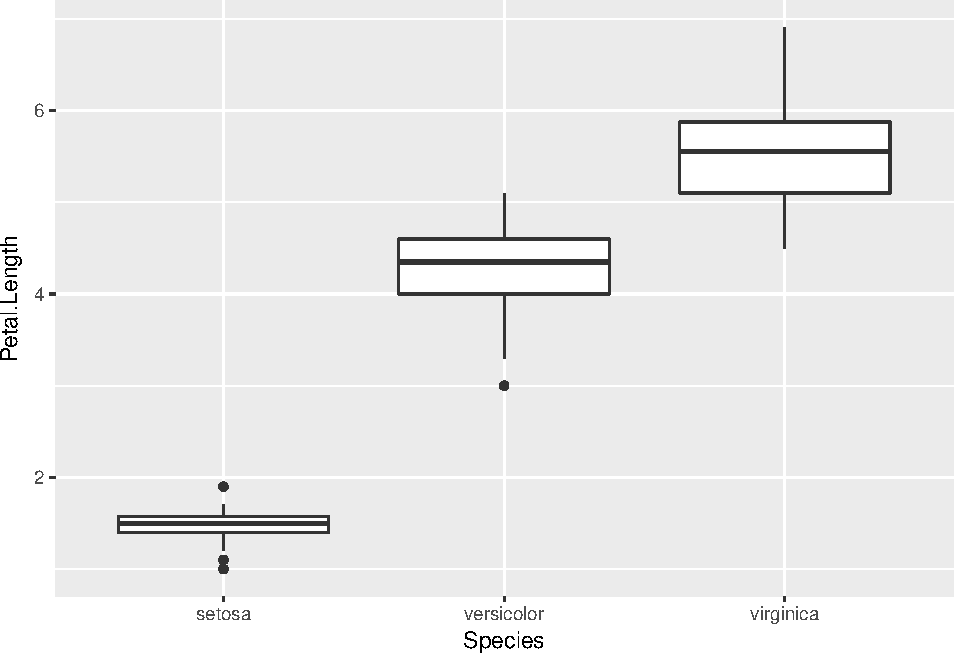
\includegraphics{Guia2_files/figure-latex/unnamed-chunk-5-1.pdf}
\caption{Box plot del largo de petalo de tres especies del género Iris}
\end{figure}

En los Box Plots tenemos 4 visualizaciones:

\begin{itemize}
\tightlist
\item
  Mediana (linea grueza)
\item
  Caja (Cuantiles 25\% y 75\%)
\item
  Bigotes (intervalo de confianza del 95\%)
\item
  Puntos Outlayers
\end{itemize}

Realice un boxplot de los datos de la educación de Chile, ¿Qué nos dice
esto de los datos?

\subparagraph{Jitter plot}\label{jitter-plot}

El jitter plot suma un punto por cada observación, lo cual nos permite
entender un poco más la naturaleza de los datos. En general se le agrega
a un box plot para tener mayor claridad en los datos (Figura 2).

\begin{Shaded}
\begin{Highlighting}[]
\KeywordTok{data}\NormalTok{(}\StringTok{"iris"}\NormalTok{)}
\KeywordTok{ggplot}\NormalTok{(iris, }\KeywordTok{aes}\NormalTok{(}\DataTypeTok{x =}\NormalTok{ Species, }\DataTypeTok{y =}\NormalTok{ Petal.Length)) }\OperatorTok{+}\StringTok{ }\KeywordTok{geom_boxplot}\NormalTok{() }\OperatorTok{+}\StringTok{ }\KeywordTok{geom_jitter}\NormalTok{(}\KeywordTok{aes}\NormalTok{(}\DataTypeTok{color =}\NormalTok{ Species))}
\end{Highlighting}
\end{Shaded}

\begin{figure}
\centering
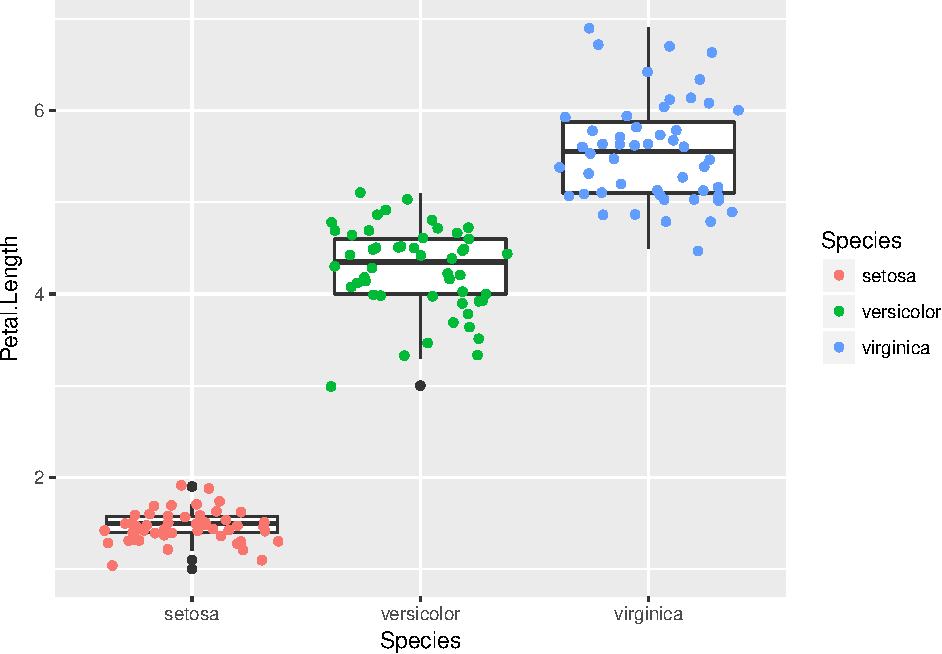
\includegraphics{Guia2_files/figure-latex/unnamed-chunk-6-1.pdf}
\caption{Box plot y jitter plot juntos para el largo de petalo de tres
especies del género Iris}
\end{figure}

\subsection{Actividad 2 Captación de CO2 en
plantas}\label{actividad-2-captacion-de-co2-en-plantas}

Utilizaremos base de datos \(CO_2\) enviada al curso. Esta base de
datos, tambien presente en R, tiene las siguientes variables

\begin{itemize}
\tightlist
\item
  \textbf{Plant}: Identidad de cada planta
\item
  \textbf{Type}: Variedad de la planta (subespecie Quebec o Mississippi)
\item
  \textbf{Treatment}: Tratamiento de la planta, algunas fueron enfriadas
  la noche anterior (Chilled)
\item
  \textbf{conc}: Concentración ambiental de \(CO_2\)
\item
  \textbf{Uptake}: Captación de \(CO_2\) para cada planta en cada día
\end{itemize}

¿Hay diferencias entre la captación de \(CO_2\) en plantas tratadas y no
tratadas?

\begin{itemize}
\tightlist
\item
  Genere tablas resumenes que le permitan explorar esta pregunta

  \begin{itemize}
  \tightlist
  \item
    ¿Existen variables que puedan confundir el resultado? ¿como trataría
    los datos para lidiar con esto?
  \end{itemize}
\item
  Genere gráficos exploratorios para contestar esta pregunta
\end{itemize}

\subsection{Actividad 3 Mi primer
ANOVA}\label{actividad-3-mi-primer-anova}

En \emph{R} todos los modelos tienen la siguiente estructura
\textbf{Funcion(y \textasciitilde{} x1 + x2 + \ldots{} + xn, data =
MisDatos)}, donde la \textbf{Funcion} dice el modelo que queremos
realizar (por ejemplo ANOVA, regresión lineal, modelos mixtos, etc.),
\textbf{y} es la variable que queremos explicar, \textbf{x1} a
\textbf{xn} son las variables explicativas, \textbf{\textasciitilde{}}
es un simbolo que debe ser leído como explicado por y finalmente
\textbf{data} es la base de datos que queremos utlizar, en un ANOVA
(análisis de varianza), la función en cuestion es aov.

En el siguiente código vemos si el largo del pétalo de las flores del
género \emph{Iris}, pueden ser explicados por la especie a la que estas
plantas pertenecen, por lo que generamos un modelo llamado
\emph{Primer.Anova} con la función \textbf{aov}.

\begin{Shaded}
\begin{Highlighting}[]
\NormalTok{Primer.Anova <-}\StringTok{ }\KeywordTok{aov}\NormalTok{(Petal.Length }\OperatorTok{~}\StringTok{ }\NormalTok{Species, }\DataTypeTok{data =}\NormalTok{ iris)}
\end{Highlighting}
\end{Shaded}

Para acceder a la tabla de resultados utilizamos la función
\textbf{summary}

\begin{verbatim}
##              Df Sum Sq Mean Sq F value Pr(>F)    
## Species       2  437.1  218.55    1180 <2e-16 ***
## Residuals   147   27.2    0.19                   
## ---
## Signif. codes:  0 '***' 0.001 '**' 0.01 '*' 0.05 '.' 0.1 ' ' 1
\end{verbatim}

Si establecemos el valor de alfa en 0.05 y al ver en la tabla que el
valor de p es menor a alfa, rechazamos la hipótesis nula de que las
medias son iguales, y decidimos que la media del largo de pétalo es
distinta entre las especies.

\subsubsection{Ejercicio}\label{ejercicio}

Determine si para la base de datos \textbf{CO2} la captación de \(CO_2\)
es distinto entre platnas con tratamiento de enfriamiento y sin
enfriamiento.


\end{document}
